\chapter{Experiments}
\lhead{\emph{Experiments}} 
\label{chap:experiments}	

\section{Experimental Setup}
\label{sec:experimentat-setup}

As depicted in figure~\ref{fig:scenario}, three robotic arms are used for the experiment. The global task is to transport all cubes available at buffers 1 ($B_1$) and 2 ($B_2$) into buffer 3 ($B_3$) with the least amount of loss possible. When a cube reaches $B_3$ it is considered \textit{sinked}. If it is lost in transit, it is considered \textit{dropped}. Drop of cubes happens in two different situations. First, a buffer already containing the maximum number of cubes (full buffer) will drop any newly added element. The second way to lose a cube is related to the way a conveyor operates. The conveyor automatically transfers cubes from its head buffer to its tail buffer in a predetermined number of time steps. It does so by moving the head buffer to the other end of the conveyor. This makes the head buffer unavailable for deposit during the transfer process. During that period of time any attempt of depositing a cube on to the conveyor will result in a dropped cube. See appendix \ref{app:arch-overview} for an in-depth look at the architecture used.  

The robotic arms can either be scripted or managed by an agent while the rest of the entities reacts automatically to the state of the environment. The number of time steps required by the conveyors to move a cube from the head to the tail buffer is set to $1$. All buffers related to the conveyors have a maximum size of $1$ while the other buffers have no maximum size.

\begin{figure}[ht]
\centering
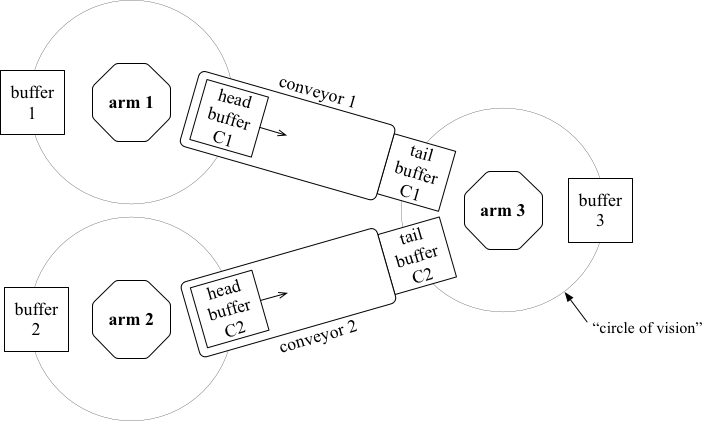
\includegraphics[width=0.7\textwidth]{imgs/scenario.png}
\caption[Scenario overview]{Schematic overview of the environment used. The figure depicts the entities involved and their relationship. The circle around the arms is referred as "the circle of vision".}
\label{fig:scenario}
\end{figure}

During the simulation and at each time step, the agents controlling the arms must select one action from their respective action space. At minimum, they all have access to the state information relative to the entities in their "circle of vision" as well as their own internal state to make their decision. The circle of vision is depicted in figure~\ref{fig:scenario} by the circle around each arm. $agent_{arm1}$ has guaranteed access to the state of $B_1$, $HBC_1$ as well as the position of the conveyor 1. Indeed, the position of the conveyor is required to know the availability status of the head buffer. The observation space of $agent_{arm2}$ is similar. $agent_{arm3}$'s observation space contains the state of $TBC_1$ and $TBC_2$ as well as the state of $B_3$. 

It is assumed that all agents have access to a \textit{noop} action indicating that the agent does not wish to execute anything.   When communication is enabled, $agent_{arm3}$ is the only agent that need to take both physical actions and communication actions. Its physical action space is composed of (1) move cube from $TBC_1$ to $B_3$, (2) move cube from $TBC_2$ to $B_3$ and (3) $noop$. The action space of the feeding $arm_i$ for $i \in {1,2}$ is composed of (1) move cube from $B_i$ to $HBC_i$ and (2) $noop$.

$arm_3$ (\textit{receiving} arm) is slower compared to the \textit{feeding} arm $arm_1$ and $arm_2$. It takes the receiving arm 3 time steps to move a cube from a point to another while for the two feeding arm, a single time step is needed. This speed disparity removes possible intrinsic coordination between the feeding and receiving arms. 

The environment will move from $t$ to $t+1$ only after all actions selected at time $t$ have been applied to the environment. The execution of a selected action might be refused. This happens if the underlying physical arm is still executing a past action. For example, at $t_0$, the agent responsible for $arm_3$ decides to take action $a$ (corresponding to moving a cube from $p_1$ to $d_1$). Because the speed of transport for $arm_3$ is $3$, the underlying arm will not be responsive to any new action during $t_1, t_2$ and $t_3$. This means that the only action the agent should select during those time steps is the $noop$ action.

\section{Communication schemes}
\label{sec:communication-schemes}

Communication can be approached from two different stand points. At each time step, beside a physical action, a communicating agent will also select a communication symbol (or message) $v \subset V \in \mathbb{R} ^{K \times 1}$. The symbols are discrete elements taken from a vocabulary $V$ of size $K$. The selected message $v$ will then be transmitted to the other agents. It is assumed that the messages in the vocabulary are distinct. Then, based on both their individual observation and the messages received, the agents will be able to select a physical action. The used communication schema influences the time between the sending of a message and its reception by the other agents. The first approach inspired by \cite{mordatch_emergence_2017} uses an instantaneous channel. A message selected at time step $t$ is directly available to the other agents. On the other hand, communication can be delayed as described by \cite{foerster_learning_2016}. With this approach, a message selected at time step $t$ will only be available to the other agent at minimum at time step $t+1$. It is important to stretch that no prior signification is assigned to the vocabulary symbols. Meaning will be assigned during training time by the agents themselves. Figure~\ref{fig:com-channels} illustrates the differences between the two communication approaches. 

\begin{figure}[ht]
\centering
  \begin{minipage}[t]{0.5\textwidth} %trying to force figs apart
    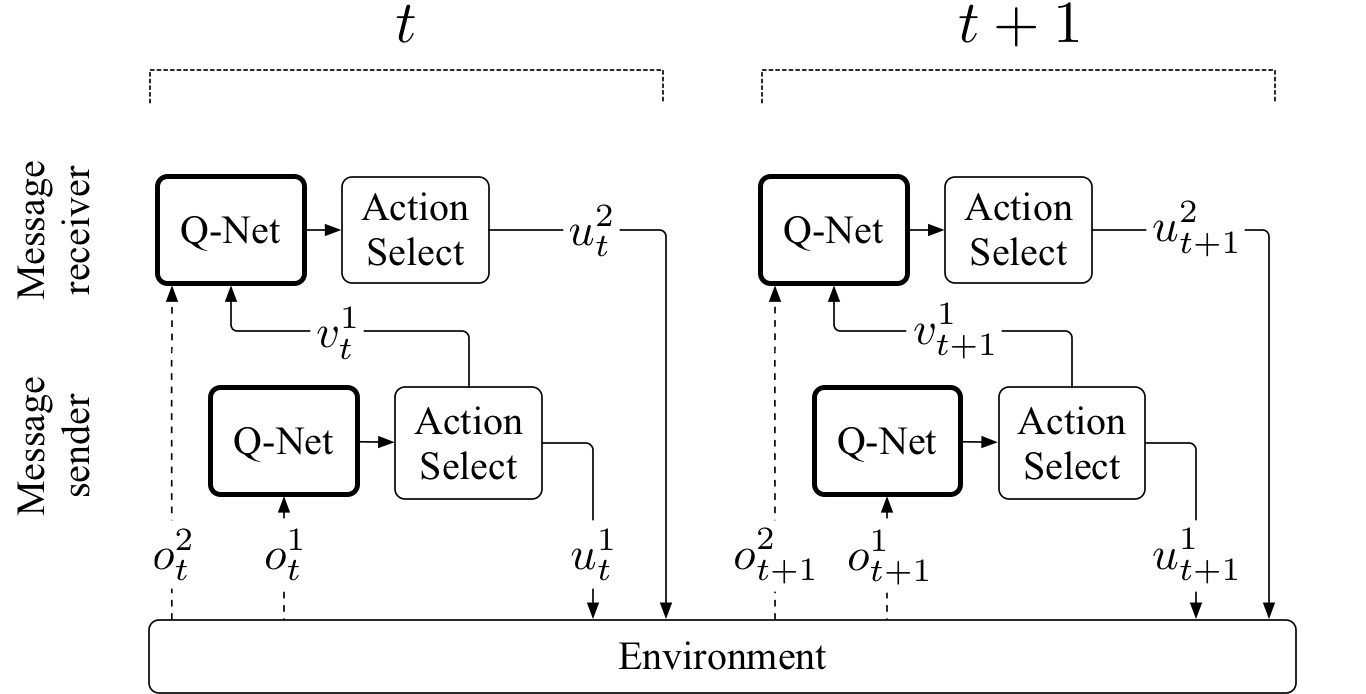
\includegraphics[width=\linewidth]{imgs/com-instant.png}
   % \caption*[Instantaneous communication scheme]{\textbf{Instantaneous communication} The message sent by a communicating agent are directly available to the other agents for their physical action selection.}
   \caption*{\textbf{Instantaneous communication} The message sent by a communicating agent are directly available to the other agents for their physical action selection.}
  \end{minipage}%
  \hfill
  \begin{minipage}[t]{0.5\textwidth}
    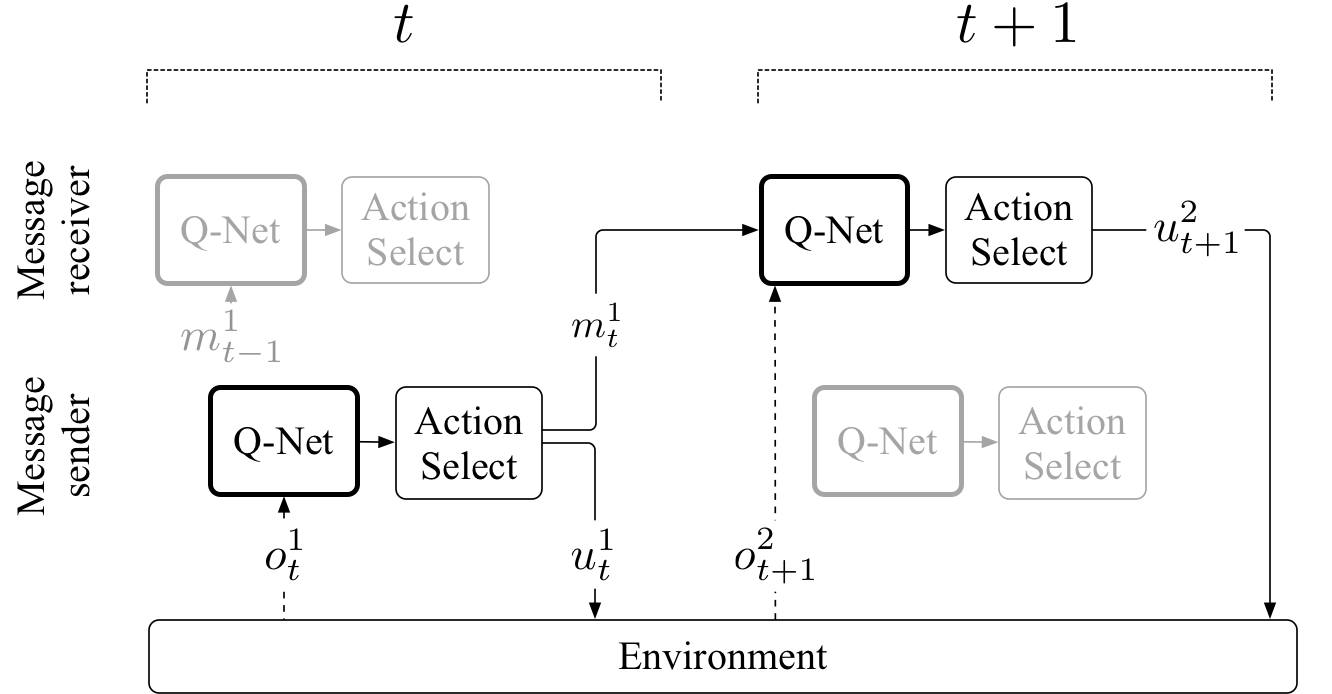
\includegraphics[width=\linewidth]{imgs/com-delay.png}
    %\caption*[Delayed communication scheme]{\textbf{Delayed communication} The message sent are available to the other agent at the following time step}
    \caption*{\textbf{Delayed communication} The message sent are available to the other agent at the following time step}
  \end{minipage}
  \caption{Comparison of process flow between instantaneous and delayed communication \protect\footnotemark}
  \label{fig:com-channels}
\end{figure}

\footnotetext{Figures are inspired by \cite{foerster_learning_2016}.}

In the experiments discussed in chapter~\ref{chap:discussion}, only $agent_{arm3}$ can communicate in a broadcast fashion to $agent_{arm1}$ and $agent_{arm2}$. Following the work of \cite{foerster_learning_2016}, $agent_{arm3}$ is separated into two sub-agents. One agent is used to select the communication action ($agent_{arm3c}$) and the other one to select the physical action ($agent_{arm3u}$). Both sub-agents share the same observation space. 

\section{Reward function}
\label{sec:reward-function}

The most straight forward reward would be related to the solving of the task. Unfortunately, initial experiments showed that this approach does not provide enough feedback to the agents to learn effectively. Instead, reward shaping is used. In order for the learner to strive for cooperative behaviour the reward signal is shared between the agents. The global reward is as follows:

\begin{equation}
    r_{t} = \sum_{a \in A_t} R(s_{t-1}, a, s_t) + r_{time}
\end{equation}

The global reward is hand-crafted from three sub-parts. As an incentive to avoid drop of cubes, a \textbf{cube reward} is added per cube transported during the time-step. A reward of $-1$ is given if the cube is dropped, $1$ otherwise. A selected action might give rise to a \textbf{behaviour reward} of $-1$ if it was not realised by the underlying arm. This signal is used to avoid flooding of the meta controller by the learners with actions that can not be fulfilled. For example, this situation can happen when the underlying arm is still moving. An additional fixed reward ($r_{time}$) is added to he global reward for every elapsed time-step. A negative \textbf{time reward} can be used to push agents to be active and finish the task as soon as possible.

\begin{equation*}
    R(s_{t-1}, a, s_t) = c(s_{t-1}, a, s_t) + b(s_{t-1}, a, s_t)\\
\end{equation*}

\begin{equation*}
\begin{array}{rl}
    c(s_{t-1}, a, s_t) = & \left\{
     \begin{array}{rl}
       -1 & : \text{action $a$ resulted in a drop of cube}\\
       +1 & : \text{action $a$ resulted in a correctly transported cube} \\
       0 & :  \text{otherwise}
     \end{array}
    \right. \\
    b(s_{t-1}, a, s_t) = & \left\{
     \begin{array}{rl}
       -1 & : \text{action $a$ was not executed (refused)}\\
       0 & :  \text{otherwise}\\
     \end{array}
   \right.
\end{array}
\end{equation*}

On top of the shared reward, a individual \textbf{communication reward} ($r_{com}$) can be added. The communication reward is related to usage cost of the channel. It might be positive to favour usage of the channel or negative to favour communication scarcity. It is assumed that the vocabulary at the disposal of a communicating agent contains an equivalent to "no message sent" which incurs no cost. This enables the learner to decide if sending a message is worth the cost.

\section{Training}

One training session is composed of 6000 episodes. An episode corresponds to one transport session happening in the environment described above. Before each episode, the world is reset. All cubes still present are removed and all robotic arms are reset. Afterwards, each buffer is filled with a random number of cubes. The number of cube put into each buffer follows a normal distribution $\mathcal{N}(\mu=0.75*\textit{max buffer size}, \sigma=3)$. An episode is considered finished either when a predetermined number of time steps has been done or when no cube are left to transport  (all cube have either reached buffer 3 or have been dropped). Chapter~\ref{chap:discussion} presents a comparison between learning scenarios as well as the influence of the different hyper parameters on the learned solutions. In order to evaluate the efficacy of the policies learned, the resulting learners are applied to $500$ new random problems. The learning process is repeated $50$ times. A solution is considered optimal if during the 500 evaluation problems 100\% of the cube to be transported reach buffer 3 ($B_3$).

\subsection*{Centralised Learning}

This approach uses a single agent making decisions based on a concatenation of all observation and action space of all agents. With this approach there is no autonomy of agents and the multi-agent task is transformed in a single agent task. The centralised learning is used as one of the baselines.

\subsection*{Decentralised Learning}

When decentralised learning is used, each arm is managed by an autonomous agent learning at the same time in the same task. Both decentralised learning with full and partial observability are explored. In order to circumvent the inability of the agents to have a direct insight about the other agent behaviours in the partial observability case, communication is used.

\subsection{Action selection and exploration}

Learners are all implemented using vanilla tabular Q-learning with optimistic initialisation. The discount factor used during learning will be indicated for each experiment. The actions are selected to be the maximum estimated Q-Value relative to a given observation, $a = \argmax_a q(o, a)$. In order to maintain exploration during training, an $\epsilon$-greedy policy is used with an exploration rate decreasing linearly over time from 0.5 to 0.05.













% # Instantaneous communication analysis

% ## Perfect channel
% Table Optimality (rwdt, disc + costless com)
% Optimality per variable (rwdt, disc + costless com)

% Table com-compelexity (rwdt, disc + costless com)
% Com-complexity per variable (rwdt, disc + costless com)

% Grounding of communication:
% - Look only at optimal resolutions

% Usage of zero by AC based on communication cost state [1,1], [1,0], [0,1] (can receive) make into relation with number of optimal
% Reaction to message i.e. meaning of received message


% # SIMULATION TO DO
% ## Unperfect channel (drop)
% - Drop rate (best disc, best com-r, best time-r)
% - Com-msg (2,3,4,8)


% -  MARLAO Busoniu p21 for justification for Q-Learning



